\documentclass{article}

% If you're new to LaTeX, here's some short tutorials:
% https://www.overleaf.com/learn/latex/Learn_LaTeX_in_30_minutes
% https://en.wikibooks.org/wiki/LaTeX/Basics

% Formatting
\usepackage[utf8]{inputenc}
\usepackage[margin=1in]{geometry}
\usepackage[titletoc,title]{appendix}

% Math
% https://www.overleaf.com/learn/latex/Mathematical_expressions
% https://en.wikibooks.org/wiki/LaTeX/Mathematics
\usepackage{amsmath,amsfonts,amssymb,mathtools}

% Images
% https://www.overleaf.com/learn/latex/Inserting_Images
% https://en.wikibooks.org/wiki/LaTeX/Floats,_Figures_and_Captions
\usepackage{graphicx,float}

% Tables
% https://www.overleaf.com/learn/latex/Tables
% https://en.wikibooks.org/wiki/LaTeX/Tables

% Algorithms
% https://www.overleaf.com/learn/latex/algorithms
% https://en.wikibooks.org/wiki/LaTeX/Algorithms
\usepackage[ruled,vlined]{algorithm2e}
\usepackage{algorithmic}

% Code syntax highlighting
% https://www.overleaf.com/learn/latex/Code_Highlighting_with_minted
\usepackage{listings}
%\usepackage{minted}
%\usemintedstyle{borland}

\usepackage{hyperref}
\usepackage{subcaption}
\usepackage{bm}

% References
% https://www.overleaf.com/learn/latex/Bibliography_management_in_LaTeX
% https://en.wikibooks.org/wiki/LaTeX/Bibliography_Management
%\usepackage{biblatex}
%\addbibresource{references.bib}

% Title content
\title{AMATH 582 Homework Three: Principal Component Analysis}
\author{Daniel W. Crews}
\date{February 24, 2021}

\begin{document}

\maketitle

% Abstract
\begin{abstract}
  Measurements generically include superfluous components (from the perspective of an analyst at least). An old, efficient, and quite spectacular method to extract particular dynamics within a dataset is called principal component analysis (PCA). Basically, PCA is an eigendecomposition of the covariance matrix. This report utilizes PCA to analyze simple harmonic motion recorded on separate video cameras, assigning different oscillatory components to particular modal coordinates rather their motional ones. %rather than dispersed between various different ones. % Spectral analysis consists of far more than determination of the Fourier coefficients of a time series. This numerical experiment explores the spatial distribution of a signal's frequency spectrum (or spectrogram) through the pratical examples of classic shredding moments in music history (here, Guns and Roses and Pink Floyd). To compute the spectrograms a short-time (masked) Fourier transform is used, and in particular this report explores its filtering using the Wigner distribution function of the time series. Here the Wigner function is computed as an $\mathcal{O}(N^2)$ operation in terms of the Fourier coefficients.
    %Signal processing is used ubiquitously in science and engineering. This simple numerical experiment explores an important aspect of signal analysis, namely statistical averaging of a spectral time series to eliminate noise and thereby identify center frequencies. Here the time series consists of a spatial wavefield which is denoised via Gaussian filtering about the identified frequency to determine a trajectory. While the technique explored in this report is quite elementary compared to more sophisticated signal processing approaches, it conveys the essential elements of, for example, a radar or sonar tracking system. %In this case such a trajectory is determined from a noisy waveform in a time series of three spatial dimensions. 
\end{abstract}

% Introduction and Overview
\section{Introduction and Overview}
Here four experiments are analyzed of videos taken from three perspectives of a mass oscillating at the end of a string. The four experiments consisted of simple one-dimensional harmonic motion in gravity from the string tension, then introduction of an additional swinging pendulum motion, and thirdly also rotation of the oscillating mass. Finally data was collected with camera shake in order to introduce measurement noise. The measurements are composed of multiple relatively independent simultaneously occuring oscillations to demonstrate the mathemagical properties of the principal component analysis (PCA) method, which separates oscillatory modes by an eigendecomposition (thus, diagonalization) of the data covariance matrix.

%The purpose of this work is to visualize some of the most famous shredding in rock and roll history (Pink Floyd and Guns and Roses (GNR)) by construction of a spectrogram. Section \ref{theory} outlines the theory of the combined Gabor-Wigner distribution used for the spectrogram, followed by a section detailing implementation of the algorithm. Results are presented for the opening guitar riff in GNR, bass line in Floyd, and a stab at the Floyd guitar solo. The attached appendices describing elements of Wigner distributions are hoped not to count towards the overall page limit and included merely for completeness. The report itself is kept concise.

% This report describes an algorithm used to denoise the signal via a statistical method and to identify the submarine's trajectory. It begins with a brief theoretical overview of the methods used, and proceeds to a discussion of the details of the code used to implement the methods. There is then a discussion of results identifying the three-dimensional trajectory, along with a suggested search area for a submarine-tracking aircraft and the likely frequency of the submarine. The report is kept brief without sacrificing clarity.

% Theoretical Background
\section{Theoretical Background}\label{theory}
\subsection{Principal component analysis}
Any particular data matrix $X\in\mathbb{C}^{m\times n}$ has an associated covariance matrix \cite{kutz}
\begin{equation}
  \mathcal{C}_X = \text{cov}(X) \equiv \frac{1}{n-1}(\delta X)(\delta X^\dagger)
\end{equation}
where $\delta X = X - \langle X\rangle$. Each component $\mathcal{C}_{ij}$ expresses the covariance $\langle\langle X_{ik}X^*_{kj}\rangle\rangle \equiv \langle (X_{ik} - \langle X\rangle)(X_{kj} - \langle X\rangle)^*\rangle$, or correlation coefficient of the component $X_{ij}$ in relation to the entire dataset\footnote{Geometrically, the inner product of components represents a correlation by measuring the extent of their alignment.}. Note that in the case of complex data one may also split the component vectors of $X$ into real and imaginary parts and calculate a real correlation matrix between those components with doubled dimension. For example, a complex function $\psi(t)$ with autocorrelation function $\kappa(\tau) = \langle\langle \psi(0)^*\psi(\tau)\rangle\rangle$ has relation to its $2\times 2$ autocorrelation matrix $K$,
\begin{equation}
\kappa(\tau) = K_{00} + K_{11} + i(K_{01} - K_{10}).
\end{equation}
Note that $\kappa(\tau)$ has reduced information from $K(\tau) = \text{cov}(\{\text{Re}(\psi),\text{Im}(\psi)\})$ \cite{vankampen}. Now $X$ represents a linear operation between vector spaces $\mathbb{V}^m\to\mathbb{V}^n$. However, $\text{cov}(X)\in\mathbb{C}^{m\times m}$ is by definition self-adjoint. Therefore its eigenvalues are distinct and there exists a choice of basis $q\in\mathbb{V}$ diagonalizing $\text{cov}(X)$,
\begin{equation}
  (\delta X)(\delta X^\dagger) = Q\Lambda Q^{-1}
\end{equation}
where $\Lambda$ is the diagonal of eigenvalues and $Q$ is unitary. In the projected variable $Y = Q^TX$, $\text{cov}(Y) = \frac{1}{n-1}\Lambda$, so that these \textit{principal components} $Y$ represent the data in a decorrelated basis.%Note that this conclusion is only possible if the system is diagonalizable (in the case of irreducible correlation or intrinsic uncertainty complete diagonalization is not possible and is only an approximation, such as in quantum theory).

\subsubsection{Singular value decomposition}
A limitation of the eigenvalue approach is that the matrix $X$ itself may not be square and so not diagonalizable in that particular sense. The generalized eigendecomposition/diagonalization of $X$ is called the \textit{singular value decomposition} (SVD). The idea is to measure the action of $X$ on vectors $V$ spanning a unit hypersphere in the base space into unit vectors $U$ of resultant lengths $\Sigma$ tracing a hyperellipse in the target space,
\begin{equation}
  XV = U\Sigma,\quad V^{-1} = V^\dagger,\quad\implies\quad X = U\Sigma V^\dagger
\end{equation}
In this picture $U\in\mathbb{C}^{m\times n}$, but in most implementations $m-n$ additional orthonormal columns are added to make it square $m\times m$ (i.e. through Gram-Schmidt procedure), and thus $\Sigma$ is a diagonal $m\times n$ matrix with silent $m-n$ rows (possibly more if rank $r$ of $X$ is less than $n$). As matrices of orthonormal basis vectors both $U$ and $V$ are unitary. The stretching components $\Sigma$ are called $\textit{singular values}$, apparently here in the sense of ``particular'' or ``characteristic'' rather than ``explody singular''.

As a generalized eigendecomposition the direct SVD of $X$ also accomplishes diagonalization of the covariance matrix $\text{cov}(X)$ by representing the \textit{two} characteristic problems of $X$ in the case $m\neq n$, \cite{kutz}
\begin{align}
  X^\dagger XV &= V\Sigma^2,\\
  XX^\dagger U &= U\Sigma^2.
\end{align}
The latter guarantees diagonal covariance of the projected variable $Y = U^\dagger X$, as $\text{cov}(Y) = \frac{1}{n-1}\Sigma^2$.

% Algorithm Implementation and Development
\section{Algorithm Implementation and Development}\label{section}
The provided data consists of color video frames. The RGB color was first mapped to grayscale in order to work with scalar data. For each of the four data sets the video frames were then synchronized in time to equal frame-lengths by choosing start and end frames by eye. As a first reduction of the data to its relevant parts, coordinates of the bucket (oscillating mass) then had to be tracked. The first attempt at bucket tracking consisted of calculating temporal differences (effectively a differentiation). This differencing procedure was noisy and unreliable for the shaky camera, so a method based on ``color filtering'' was utilized.

The color filtering method starts with the observation that the brightest part of the image is mostly the white paint-bucket, so the grayscale camera dataset can be set to zero below a certain brightness threshold using masking notation, \texttt{cam1[cam1 <= t] = 0} where \texttt{cam1} is the dataset and \texttt{t} the threshold value (for example, with a maximum grayscale value of $255$, \texttt{t}$\sim 240$ was appropriate). As other bright spots happened to be on the periphery of the camera field-of-view, these values were then masked to zero manually (see Fig. \ref{masked_bucket} for example). The $(x,y)$ trajectory of the bucket was then found using the mean coordinates of all points above the threshold per frame, e.g. \texttt{np.mean(X[np.where(cam[:,:,i] > 0)])} where \texttt{X} is a meshgrid of x-pixel coordinates. Finally, as there are fluctuations per frame in the particular parts of the bucket passing the color filter, the coordinates are smoothed with a moving average filter (typically three-five frames).

\begin{figure}[b!]
  \centering
  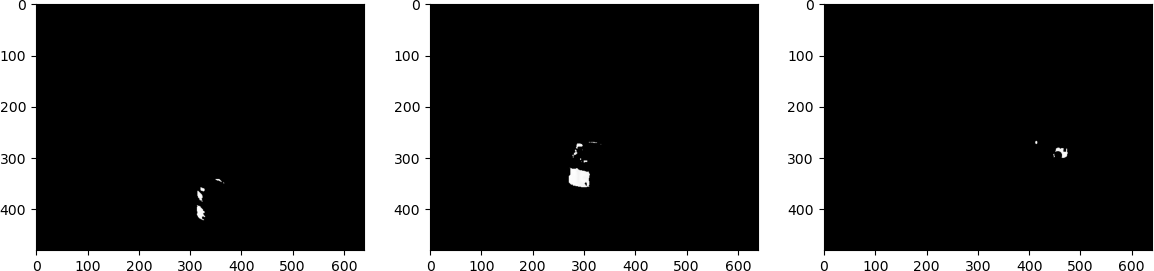
\includegraphics[width=\textwidth]{noshake_bucket}
  \caption{Appearance of the bucket in first dataset (no shake) after intensity masking.}\label{masked_bucket}
\end{figure}

After the coordinates were determined, the data matrix was assembled as $X = \{x_1; y_1; \cdots\}$, its SVD calculated (of $\delta X=X - \langle X\rangle$), and the projected components $Y = U^TX$ plotted (just transpose as the data is real-valued). For datasets with multiple oscillation components FFTs were done to compare frequencies.
% Development of the analysis algorithm proceeded as follows. The provided musical waveforms are considered to be periodic and analyzed by discrete Fourier transform. After picking out an appropriate frequency range (\textit{e.g.} the bass line in Floyd), the waveform is both Wigner and Gabor transformed, where only the analytic signal (or real FFT) is used in order to reduced to reduce low-frequency interference in the Wigner function (c.f. Section \ref{analytic}). The two phase space distributions are then multiplied together and the (logarithm of) the resulting spectrogram plotted as filled contours. Implementation details are in Appendices \ref{functions} and \ref{implementation}.

% Having obtained the spectrogram, the musical score is then reconstructed by first listening to the recording to figure out the time signature (both are 4-4). Then the frequencies are compared to a music scale chart to figure out which notes they correspond to. Finally, the score is written down. Note that the Gabor transform is sufficient for the purposes of this assignment, however the combined Wigner-Gabor spectrogram is of interest by revealing harmonic combinations (additional spectral lines) in the music. Github repository for this work is available .

\begin{figure}[t!]
  \centering
  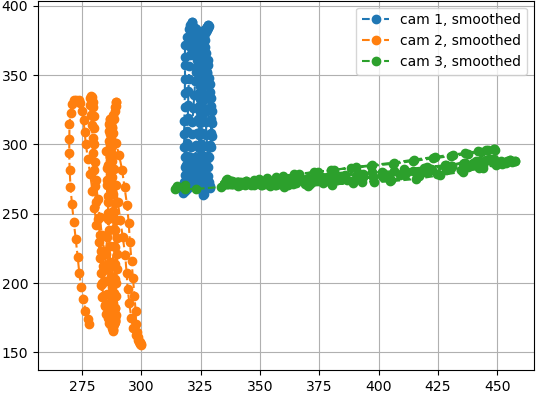
\includegraphics[width=0.31\textwidth]{noshake_traj2}\quad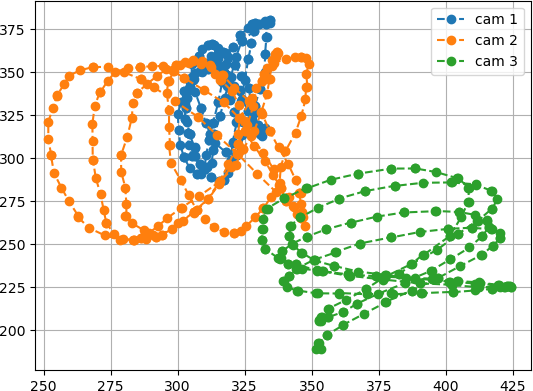
\includegraphics[width=0.31\textwidth]{pendulum_traj}\quad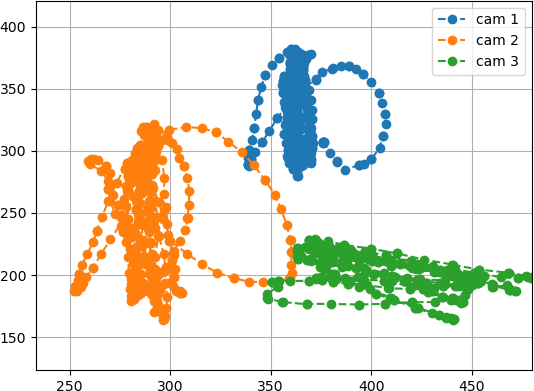
\includegraphics[width=0.31\textwidth]{rotate_coords}
  \caption{Bucket coordinates of three perspectives superimposed, with x and y axes pixels (arb. units).\\Left: Base case, SHM with no shake. Middle: SHM plus pendulum motion. Right: SHM plus bucket spin.}\label{coords}
\end{figure}

\begin{figure}
  \centering
  \includegraphics[width=0.45\textwidth]{pca_noshake3}\quad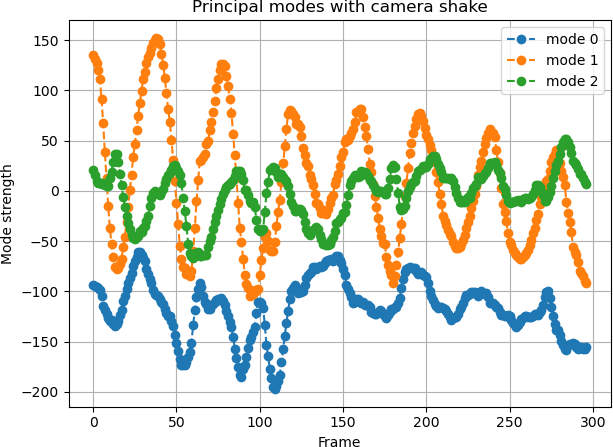
\includegraphics[width=0.45\textwidth]{pca_shake2}
  \caption{Projected modes $Y = U^TX$ for the bucket coordinates without (left) and with (right) camera shake. The six modes account for the three camera perspectives of two coordinates per frame. Evidently the oscillatory signature appears in the first dynamic mode, as the zeroth mode (a sort of DC component) describes the general location of the mass in the principal frame. It's clear that the addition of noise (right) splits the oscillation signature across different modes as they can no longer be ``perfectly'' decorrelated.}\label{sns}
\end{figure}

\section{Computational Results}
Figure \ref{coords} shows the results of tracking the bucket coordinates for the cases of simple harmonic motion (SHM) with no camera shake, with pendulum motion, and then with rotational motion. The case of camera shake is not shown for brevity, but is of course much noisier than any of these three cases. Then, Fig. \ref{sns} shows the PCA results for the baseline case (no camera shake) and with shake. According to the results, oscillation appears at first-order in the decorrelation and the addition of noise smears the oscillatory signature across multiple modes. This makes intuitive sense as noise ought to prevent ideal decorrelation of data components.

Finally Fig. \ref{pr} shows the results of PCA on the SHM first with superimposed pendulum oscillation and secondly with bucket rotation. The interesting and seemingly magical result (with mathematical foundations of course, cf. Section \ref{theory}!) is that the separate oscillatory components are well separated in the decorrelation. Some interference (weak modal coupling) is to be expected to hamper decorrelation, and this is perhaps seen in the zeroth mode (however this is merely speculation). FFTs on these datasets are not shown for conciseness, as the largest amplitude frequencies are clearly visible. However, one is shown in Fig. \ref{pend_fft} to demonstrate that the ``mode 0'' waveform of the pendulum dataset is indeed composed of both frequencies.

\begin{figure}[h]
  \centering
  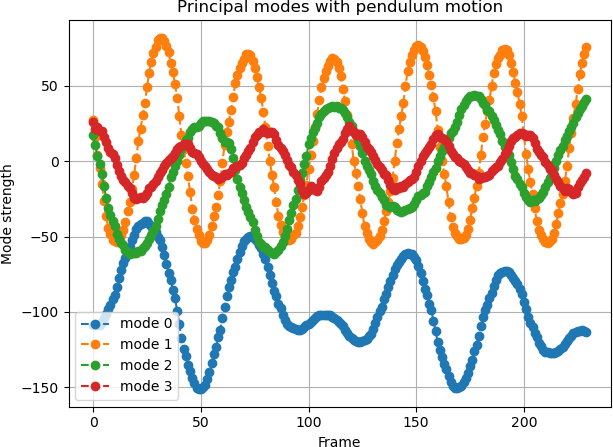
\includegraphics[width=0.45\textwidth]{pca_pend2}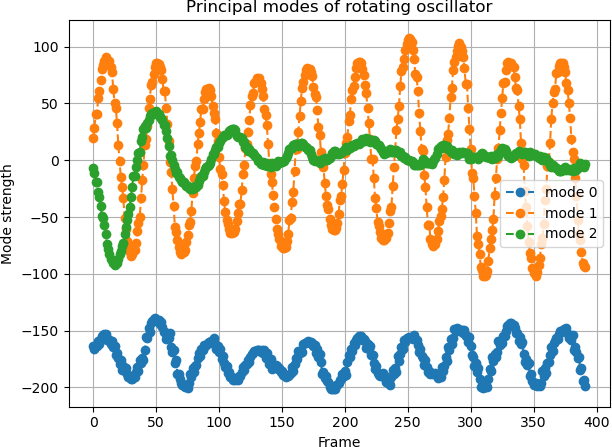
\includegraphics[width=0.45\textwidth]{pca_rotate2}
  \caption{Projected modes of bucket coordinates for cases of SHM superimposed on pendulum motion (left) and bucket rotation (right). In comparison to the baseline case (Fig. \ref{sns}) clearly ``mode 1'' still describes the bucket SHM as their frequencies match. The pendulum motion appears as a lower-frequency oscillation apparently in ``mode 2''. However, the occurence of both oscillations appears to leave a modulated trace (superposition?) in mode 0, in curious correlation with the Wigner function experiments of the last homework. The rotating oscillator case shows a damped rotation tendency in ``mode 2,'' matching the video here.}\label{pr}
\end{figure}

\begin{figure}[hb!]
  \centering
  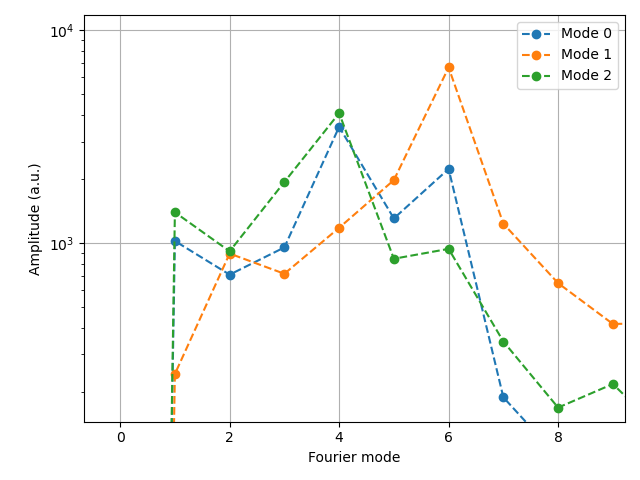
\includegraphics[width=0.5\textwidth]{pendulum_fft3}
  \caption{First few Fourier components from FFT of the pendulum case, showing the frequencies in the ``mode 0'' waveform to be the SHM and pendulum frequencies 4 and 6, and perhaps interference in mode 5.}\label{pend_fft}
\end{figure}

% \begin{table}[b]
%   \centering
%   \begin{tabular}{|l|l|l|l|l|l|l|l|l|}
%     \hline
%     Time {[}hr{]}   & 0-3.5 & 3.5-7.0 & 7.0-10.5 & 10.5-14.0 & 14.0-17.5 & 17.5-21.0 & 21.0-24.5 & All-time average \\ \hline
%     $\langle k_x\rangle_T$ {[}1/L{]} & 0.814 & 0.661   & 0.784    & 0.760     & 0.810     & 0.728     & 0.802     & 0.766            \\ \hline
%     $\langle k_y\rangle_T$ {[}1/L{]} & 0.271 & 0.292   & 0.331    & 0.240     & 0.341     & 0.267     & 0.271     & 0.288            \\ \hline
%     $\langle k_z\rangle_T$ {[}1/L{]} & -1.00 & -1.03   & -1.09    & -1.06     & -1.13     & -1.07     & -1.1125   & -1.07            \\ \hline
%   \end{tabular}
%   \caption{Observed center frequencies of data following spectral averaging over time intervals of $3.5$ hours, with seven samples per interval, then used as the filter frequencies $k_0$ in the Gaussian filter. The arbitrary spatial unit is given as $L$, not to be confused with domain length. The all-time average is given as well.}\label{frequencies}
% \end{table}

% Note that in Table \ref{frequencies} negative wavenumbers are used as the given spatial data is complex, meaning that the reality condition is not satisfied, instead $\hat{f}(-k) = \hat{f}^*(k)$ in this dataset. The absolute value is reported as ``the frequency'' of the submarine, however. This identifies the submarine's spectral signature as $\bm{k} \approx \{0.766 \pm 0.05, 0.288 \pm 0.03, 1.07 \pm 0.04 \}$ {[}1/L{]} by mean and standard deviation of the window averages of Table \ref{frequencies}, where L is an arbitrary space unit corresponding to that of the provided data, \textit{not} the domain length. The width of the space or frequency ``submarine Gaussian'' was not measured for ease of analysis.

% Having computed the center frequencies, the spectrum was filtered and the trajectory determined according to the schematic Steps 4 and 5. The resulting 3D trajectory and top-down position given in Figs. \ref{traj:3d}, \ref{traj:2d} respectively. This suggests the submarine is currently located around $\bm{x}\sim(-5, 6.5)$ in $(x,y)$.

% \begin{figure}[hb]
%   \centering
%   \begin{subfigure}{0.42\textwidth}
%     \centering
%     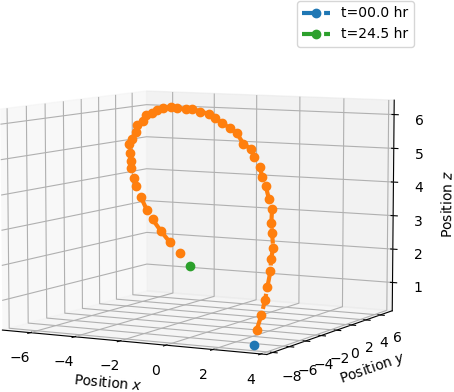
\includegraphics[width=0.99\linewidth]{pics/3d_traj}
%     \caption{Three-dimensional trajectory of submarine, showing a rise and dive maneuver.}\label{traj:3d}
%   \end{subfigure}
%   \begin{subfigure}{0.42\textwidth}
%     \centering
%     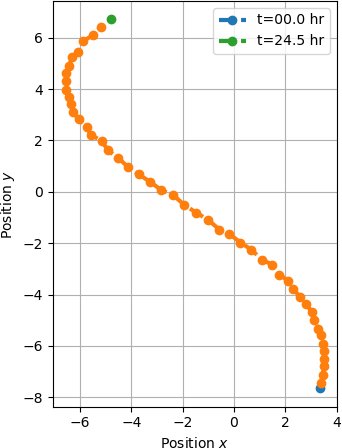
\includegraphics[width=0.6\linewidth]{pics/2d_traj}
%     \caption{Top-down view of predicted trajectory. Ideal search area for submarine-tracking aircraft is around $\bm{x} \sim (-5, 6.5)$ and continuing north-east.}\label{traj:2d}
%   \end{subfigure}
%   \caption{Identified submarine trajectory sampled 49 times in a 24.5 hour period, in 3D and 2D projections.}
% \end{figure}

% Summary and Conclusions
\section{Summary and Conclusions}
This numerical experiment analyzed video clips of some household oscillations (tensile string oscillation and gravity pendulum) as illustration of how awesome the principal component analysis method is and the usefulness of singular value decomposition. The author learned a great deal about this subject in the exercise, having never done an SVD before, and is very grateful for the learning opportunity. Theory was combined with image processing techniques to explore an analytical tool with broad scientific applications. As usual, Python was used for all implementations in this exercise and may be found at the author's Github page \href{https://github.com/crewsdw/amath582}{here}

% References
\bibliographystyle{unsrt}
\bibliography{references}

% Appendices
\begin{appendices}

\newpage
% MATLAB Functions
\section{Python Functions}\label{functions}
The following list compiles important Python functions used in implementation:
\begin{itemize}
\item The masking capability \texttt{array[bool condition] = x} is used to isolate bright parts of the image,
\item The nice concise expression \texttt{np.mean(Y[np.where(m1[:,:,i]>0)])} is used to find the mean Y values of parts of the camera array \texttt{m1} which passed the color filter, where \texttt{X,Y=np.meshgrid(x,y)} and the coordinates are taken to be \texttt{x = np.linspace(0, m1.shape[0])},
\item \texttt{u, s, vh = np.linalg.svd(X, full\_matrices=True)} is used to compute the full SVD of the data matrix after setting \texttt{X -= np.mean(X)} for covariance analysis.
\end{itemize}

% MATLAB Codes
\section{Python Implementation}\label{implementation}
A separate analysis script was used for each dataset and the files are quite similar. Only pendulum is shown for brevity (see Github page for other files).
% Wigner function file \texttt{fourier.py}:
\lstinputlisting{wpendulum.py}
% \vspace{5cm}
% Main implementation file \texttt{hw2.py}:
% \lstinputlisting{hw2.py}
% \begin{listing}[h]
% \inputminted{matlab}{example.m}
% \caption{Example code from external file.}
% \label{listing:examplecode}
% \end{listing}

\end{appendices}

\end{document}